\documentclass{beamer}

\mode<presentation>
{
  %\usetheme{CambridgeUS}
  %\usetheme{Frankfurt}
  \usetheme{Singapore}
  %\usecolortheme{crane}
  \usefonttheme{professionalfonts}
  %\usefonttheme[onlymath]{serif}
  
  \setbeamertemplate{blocks}[rounded][shadow=true]
}

\usepackage{pgfpages}

\usepackage{alltt,verbatim,amsmath,times,empheq}
\usepackage{bm}
\usepackage[english]{babel}
\usepackage[utf8]{inputenc}

%\usepackage{times}
%\usepackage[T1]{fontenc}
% Or whatever. Note that the encoding and the font should match. If T1
% does not look nice, try deleting the line with the fontenc.

%\usepackage{hyperref}

\usepackage{multimedia,xmpmulti}

\usepackage{animate}

\definecolor{dark red}{HTML}{E41A1C}
\definecolor{dark green}{HTML}{4DAF4A}
\definecolor{dark violet}{HTML}{984EA3}
\definecolor{dark blue}{HTML}{084594}
\definecolor{dark orange}{HTML}{FF7F00}
\definecolor{light blue}{HTML}{377EB8}
\definecolor{light red}{HTML}{FB9A99}
\definecolor{light violet}{HTML}{CAB2D6}

\setbeamercolor{boxed}{fg=black,bg=uaf yellow}

\newcommand{\CC}{\mathbb{C}}
\newcommand{\NN}{\mathbb{N}}
\newcommand{\RR}{\mathbb{R}}
\newcommand{\ZZ}{\mathbb{Z}}
\newcommand{\Acal}{\mathcal{A}}
\newcommand{\Bcal}{\mathcal{B}}
\newcommand{\Ccal}{\mathcal{C}}
\newcommand{\Ncal}{\mathcal{N}}
\newcommand{\Kcal}{\mathcal{K}}

\newcommand{\bF}{\mathbf{F}}
\newcommand{\bQ}{\mathbf{Q}}
\newcommand{\bU}{\mathbf{U}}
\newcommand{\bbU}{\bar{\bU}}
\newcommand{\bu}{\mathbf{u}}
\newcommand{\bv}{\mathbf{v}}
\newcommand{\bx}{\mathbf{x}}

\newcommand{\Div}{\nabla\cdot}
\newcommand{\eps}{\epsilon}
\newcommand{\grad}{\nabla}
\newcommand{\lap}{\triangle}
\DeclareMathOperator{\trace}{tr}
\renewcommand{\bar}{\overline}

\newcommand{\ddx}[1]{\frac{\partial #1}{\partial x}}
\newcommand{\ddy}[1]{\frac{\partial #1}{\partial y}}
\newcommand{\pp}[2]{\frac{\partial #1}{\partial #2}}
\newcommand{\ppt}[1]{\frac{\partial #1}{\partial t}}
\newcommand{\ppT}[1]{\frac{\partial #1}{\partial T}}
\newcommand{\ppx}[1]{\frac{\partial #1}{\partial x}}
\newcommand{\ppy}[1]{\frac{\partial #1}{\partial y}}
\newcommand{\ppz}[1]{\frac{\partial #1}{\partial z}}
\newcommand{\ppxx}[1]{\frac{\partial^2 #1}{\partial x^2}}
\newcommand{\ppzz}[1]{\frac{\partial^2 #1}{\partial z^2}}

\newcommand{\Tnorm}[1]{\left|\!\left|\!\left|#1\right|\!\right|\!\right|}
\newcommand{\rhow}{\rho_{\text{w}}}
\newcommand{\Wq}{W^{1,q}(\Omega)}
\newcommand{\half}{\frac12}

%\setbeamercolor{redtext}{fg=red!80!black}
\setbeamercolor{redtext}{fg=red!94!black}
%\setbeamercolor{greentext}{fg=green!80!black}
\setbeamercolor{greentext}{fg=green!60!black}
%\setbeamercolor{bluetext}{fg=blue!70!black}
\setbeamercolor{bluetext}{fg=blue!90!black}
\setbeamercolor{yellowtext}{fg=yellow!95!black}
\setbeamercolor{orangetext}{fg=yellow!50!red}

\newcommand{\green}{\usebeamercolor[fg]{greentext}}
\newcommand{\blue}{\usebeamercolor[fg]{bluetext}}
\newcommand{\red}{\usebeamercolor[fg]{redtext}}

\renewcommand{\L}{\emph{Left}}
\newcommand{\R}{\emph{Right}}


% this slide reappears so it is a 4/5 argument function
\newcommand{\whatvi}[4]{\longwhatvi{#1}{#2}{#3}{#4}{}}
\newcommand{\longwhatvi}[5]{
\begin{frame}
  \frametitle{what is a \emph{variational inequality}?}

\begin{enumerate}
#1{\item cute way to rewrite a calc problem in $\RR^1$; min $f$ solves:
   $$u: \qquad f'(u) (v - u) \ge 0 \qquad \text{ for all } v \in [a,b]$$}
\vspace{-4mm}
#2{\item dot-product for projection on a closed, convex $K\subset \mathcal{H}$:
   $$y=\Pi x: \qquad (y - x) \cdot (\eta - y) \ge 0 \,\, \text{ for all } \eta \in K$$}
\vspace{-4mm}
#3{\item rewriting of ``min $f$ on convex $K\subset \RR^n$'':
   $$u: \qquad \grad f (u) \cdot (v - u) \ge 0 \qquad \text{ for all } v \in K$$}
\vspace{-4mm}
#4{\item gets existence for \emph{any} continuous nonlinear eqns on 

compact, convex $K\subset \RR^n$:
   $$x: \qquad F(x) \cdot (y - x) \ge 0 \qquad \text{ for all } y \in K$$}
\vspace{-4mm}
#5
\end{enumerate}
\end{frame}
}


\title[what is \dots a variational inequality]{What is \dots a \emph{variational inequality}?}

\author[Bueler]{Ed Bueler}

\institute[UAF]{
  \tiny Dept of Mathematics and Statistics and Geophysical Institute \\

  University of Alaska Fairbanks
}

\date{\tiny 30 January, 2014}


\setbeamerfont{date}{size=\scriptsize}

\subject{variational inequality}


%\begin{comment}
\AtBeginSection[]
{
  \begin{frame}<beamer>
    \frametitle{Outline}
    \tableofcontents[currentsection,hideallsubsections]
  \end{frame}
}
%\end{comment}


\begin{document}
\graphicspath{{../commonfigs/}}

\begin{frame}
  \titlepage
\end{frame}


% NO OUTLINE BECAUSE ONE APPEARS AT START OF EACH SECTION:
%\begin{comment}
%\begin{frame}
%  \frametitle{Outline}
%  \tableofcontents[hideallsubsections]
%  % You might wish to add the option [pausesections]
%\end{frame}
%\end{comment}


\begin{frame}
  \frametitle{what is \dots \,the source of my title?}

\begin{center}
\includegraphics[height=0.205\textheight]{what-is-grobner}

\includegraphics[height=0.2\textheight]{what-is-quasimorphism}

\includegraphics[height=0.2\textheight]{what-is-random-matrix}

\includegraphics[height=0.195\textheight]{what-is-systole}
\end{center}
\end{frame}


\section[problems]{problems you can write as variational inequalities}

\begin{frame}
  \frametitle{calculus I problem}

\begin{center}
\includegraphics<1>[height=0.5\textheight]{calcprob_bare.png}
\includegraphics<2>[height=0.5\textheight]{calcprob_soln.png}
\end{center}

\begin{itemize}
\item suppose you have a smooth function \uncover<2>{\emph{on a closed, bounded interval }}
\item and you want to minimize it
\end{itemize}

\end{frame}


\begin{frame}
  \frametitle{calculus I problem}

\begin{center}
\includegraphics[width=0.33\textwidth]{calcprob_soln_interior.png}
\includegraphics[width=0.33\textwidth]{calcprob_soln_leftendpoint.png}
\includegraphics[width=0.33\textwidth]{calcprob_soln_rightendpoint.png}
\end{center}

\vspace{8mm}

because $f$ is smooth, you can say about the minimizer $u$ that:
\only<1>{
\vspace{1mm}

\begin{itemize}
\item if $a < u < b$ then $f'(u)=0$ \emph{or}
\item if $u = a$ then $f'(u) \ge 0$ \emph{or}
\item if $u = b$ then $f'(u) \le 0$
\end{itemize}
}
\only<2>{

the \alert{variational inequality} applies,
    $$f'(u) (v - u) \ge 0 \qquad \text{ for all } v \in [a,b]$$
}
\end{frame}

% where we stand
\longwhatvi{\visible}{\invisible}{\invisible}{\invisible}{{\vspace{-1cm}\\\centerline{the above is a \emph{necessary condition} only}}}


\begin{frame}
  \frametitle{projection onto a closed, convex set $K \subset \mathcal{H}$}

\begin{center}
\includegraphics[height=0.4\textheight]{proj_xy.png}
\end{center}

\vspace{-4mm}
Suppose $K \subset \RR^n$ is closed and convex.

(Or $K \subset \mathcal{H}$ closed and convex, where $\mathcal{H}$ is a Hilbert space.)

\bigskip

Definition.  Given $x\in\RR^n$ (or $x \in \mathcal{H}$), the unique minimizer
    $$y = \min_{z\in K} \|x-z\|$$
is the \emph{projection} of $x$ onto $K$, written $y = \Pi x$.
\end{frame}


\begin{frame}
  \frametitle{projection onto a closed, convex set $K \subset \mathcal{H}$}

\begin{center}
\includegraphics<1>[height=0.4\textheight]{proj_xy_vect.png}
\includegraphics<2>[height=0.4\textheight]{proj_xyprime_vect.png}
\end{center}

Theorem.
   $$y = \Pi x \qquad \iff \qquad (y - x) \cdot (\eta - y) \ge 0 \,\, \text{ for all } \eta \in K$$

\medskip
This is also a \alert{variational inequality}.

\medskip
\emph{Idea}.  The angle between $y-x$ and $\eta - y$ is $\le 90^\circ$ for all $\eta \in K$.
\end{frame}


% where we stand
\whatvi{\visible}{\visible}{\invisible}{\invisible}


\begin{frame}
  \frametitle{minimize $f$ on convex $K\subset \RR^n$}

\begin{columns}
\begin{column}{0.7\textwidth}
Consider a mainstream math problem:
\begin{itemize}
\item let $K \subset \RR^n$ be convex
\item let $f: \RR^n \to \RR$ be smooth ($C^1$)
\item find $u\in K$ so that $f$ is minimum?
\end{itemize}

\bigskip
\uncover<2->{Claim: if $u\in K$ minimizes $f$ then $u$ solves
   $$\grad f(u)\cdot (v-u) \ge 0 \qquad \text{ for all } v \in K$$}
\uncover<2->{which is a \alert{variational inequality}}
\end{column}
\begin{column}{0.3\textwidth}
\includegraphics<1->[width=1.0\textwidth]{constrained-opt}
\end{column}
\end{columns}
\end{frame}

\begin{frame}
  \frametitle{minimize $f$ on convex $K\subset \RR^n$}

\emph{Theorem}.  $K\subset \RR^n$ convex.  $f:\RR^n\to\RR$ smooth.

\noindent If $u\in K$ minimizes $f$ then
   $$\grad f(u)\cdot (v-u) \ge 0 \qquad \text{ for all } v \in K.$$

\emph{Proof}.  If $0\le t\le 1$ then
    $$(1-t) u + t v\in K$$
But $t=0$ is minimizer of
    $$g(t) = f\left((1-t) u + t v\right)$$
so by the ``calculus I problem'', $g'(0) \ge 0$.  By chain rule
    $$g'(t) = (\grad f)((1-t) u + t v) \cdot (-u + v)$$
so $g'(0) = (\grad f)(u) \cdot (v-u) \ge 0$. \qed
\end{frame}


\begin{frame}
  \frametitle{minimize $f$ on convex $K\subset \RR^n$}

\begin{columns}
\begin{column}{0.7\textwidth}
How about existence of $u$?

It happens if either:
\begin{itemize}
\item $K$ is compact
\item $K$ is closed and $f$ is coercive
\end{itemize}

\bigskip
\bigskip

How about uniqueness of $u$?

It happens if:
\begin{itemize}
\item $f$ is strictly convex
\end{itemize}
\end{column}
\begin{column}{0.3\textwidth}
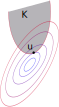
\includegraphics[width=1.0\textwidth]{constrained-opt}
\end{column}
\end{columns}
\end{frame}

% where we stand
\whatvi{\visible}{\visible}{\visible}{\invisible}


\begin{frame}
  \frametitle{solve $F(x)=0$ on $\RR^n$}

Consider another mainstream applied math problem:
\begin{itemize}
\item Given continuous function $F:\RR^n \to \RR^n$, find $x\in \RR^n$ so that
    $$F(x)=0.$$
\item That is, solve $n$ nonlinear equations in $n$ unknowns.

\vspace{5mm}
\item<2-> \emph{No one has anything positive to say about this problem:}
  \begin{itemize}
  \item[-]<2-> no guarantee of existence
  \item[-]<2-> no guarantee of uniqueness
  \item[-]<2-> no effective theory of approximation
  \end{itemize}
\end{itemize}
\end{frame}


\begin{frame}
  \frametitle{solve $F(x)=0$ on compact, convex $K\subset \RR^n$}

But we can change the problem minimally, and have something positive to say:
\begin{itemize}
\item Assume $K\subset \RR^n$ is compact and convex.
\item Seek $x\in K$ so that $F(x)=0$.
\item Theorem.  There is $x\in K$ so that
   $$F(x) \cdot (y-x) \ge 0 \qquad \text{ for all } y \in K$$
which is a \alert{variational inequality}
\end{itemize}
\end{frame}


\begin{comment}
\begin{frame}
  \frametitle{solve $F(x)=0$ on compact, convex $K\subset \RR^n$}
   $$\text{Theorem}.\quad \exists x\in K \text{ s.t.} \quad F(x) \cdot (y-x) \ge 0 \quad \text{ for all } y \in K$$
\small
\begin{itemize}
\item pick $x \in K$; generally $F(x) \ne 0$
\item let $z = x - F(x)$ and find $\Pi z \in K$
\item continuous map takes $K$ to $K$:
    $$x \mapsto \Pi (x - F(x))$$
\item Brouwer fixed point thm: $\exists x\in K$ s.t.
    $$x = \Pi (x - F(x)) = \Pi z$$
\item by previous char.~of projection,
    $$\left(\Pi z - z)\right) \cdot \left(y - \Pi z\right) \ge 0 \quad \text{ for all } y \in K$$
\item using $x = \Pi (x - F(x))$, simplify to
    $$F(x) \cdot \left(y - x\right) \ge 0 \quad \text{ for all } y \in K$$
\end{itemize}
\normalsize
\end{frame}
\end{comment}


\begin{frame}
  \frametitle{solve $F(x)=0$ on compact, convex $K\subset \RR^n$}

Theorem.  There is $x\in K$ so that
   $$F(x) \cdot (y-x) \ge 0 \quad \text{ for all } x \in K.$$

Proof. $x' \mapsto \Pi (x'-F(x'))$, as map $K\to K$, has a fixed point.
\begin{center}
\includegraphics[width=0.5\textwidth]{Fx-map-on-K}
\end{center}
\end{frame}


% where we stand
\whatvi{\visible}{\visible}{\visible}{\visible}

\begin{frame}
  \frametitle{on convex $K$}

if $K$ is convex and $u,v\in K$ and $0\le \varepsilon \le 1$ then
    $$(1 - \eps) u + \eps v = u + \eps (v-u)$$

\begin{columns}
\begin{column}{0.5\textwidth}
\includegraphics[width=1.0\textwidth]{convexview-lincomb}

$(1 - \eps) u + \eps v$ as a linear combination in $K$
\end{column}
\begin{column}{0.5\textwidth}
\includegraphics[width=1.0\textwidth]{convexview-intoK}

$u + \eps (v-u)$ as a vector from $u$ directed into $K$
\end{column}
\end{columns}
\end{frame}


\section[obstacle]{obstacle problem example}

\begin{frame}
  \frametitle{elastic membrane over obstacle}

\begin{itemize}
\item elastic membrane $z = u(x,y)$ minimizes energy
$$J[v] = \int_\Omega \frac{1}{2} |\grad v|^2 - f v$$
where $f$ is upward force on the membrane
\item if surface $v(x,y)$ is above an obstacle $\psi(x,y)$ then it's in convex set
$$\mathcal{K} = \left\{v \in H_0^1(\Omega) \,:\, v \ge \psi\right\}$$
\end{itemize}

\begin{center}
\includegraphics[width=0.35\textwidth]{figs/classicalobs} \quad \includegraphics[width=0.6\textwidth]{figs/obs-soln}
\end{center}
\end{frame}


\begin{frame}
  \frametitle{variational inequality for obstacle problem}

\begin{itemize}
\item if $u\in \mathcal{K}$ is minimizer and if $v\in\mathcal{K}$ and if $0\le \eps \le 1$ then
   \begin{align*}
   0 &\le J[u + \eps(v-u)] - J[u] \\
     &= \eps \int_\Omega \grad u \cdot \grad(v-u) - f (v-u) + \eps^2 \int_\Omega |\grad(v-u)|^2
   \end{align*}
\item thus as $\eps \to 0^+$, we know that $u\in\mathcal{K}$ satisfies
  $$\int_\Omega \grad u \cdot \grad(v-u) - f (v-u) \ge 0 \qquad \forall v\in\mathcal{K}$$
which is the variational inequality formulation
\item also written:
  $$\left<\grad J(u), v-u\right> \ge 0 \qquad \forall v\in\mathcal{K}$$
\end{itemize}
\end{frame}


\begin{frame}
  \frametitle{PDE for obstacle problem}

\small
\begin{itemize}
\item where $u>\psi$, the variational inequality implies $-\grad^2 u = f$
   \begin{itemize}
   \item[$\circ$] $-\grad^2 u = f$ is ``Poisson equation'',
   \item[$\circ$] the standard PDE for an (unobstructed) elastic membrane
   \end{itemize}
\item one can say
\begin{quote}
the membrane $u(x,y)$ solves $-\grad^2 u = f$ except when it is in contact with the obstacle
\end{quote}
\item but the set on which the contact happens is \emph{a priori} unknown \dots
\end{itemize}
\normalsize

\begin{center}
\includegraphics[width=0.55\textwidth]{figs/obs-soln} \quad \includegraphics[width=0.35\textwidth]{figs/obs-coincidence} 
\end{center}
\end{frame}


\begin{frame}
  \frametitle{finite elements}

\begin{itemize}
\item the finite element method (FEM) was built on variational \emph{equalities}, i.e.~``weak formulations''
\item so variational inequalities play well with FEM
\item FEM represents (approximates) function spaces on pretty meshes like this:
\end{itemize}

\begin{center}
\includegraphics[width=0.3\textwidth]{figs/constantineexample3}
\end{center}
\end{frame}


\begin{frame}
  \frametitle{the 3-point, one-dimensional obstacle problem}

\begin{itemize}
\item for example, consider a one-dimensional obstacle problem
\item with an equally-spaced 3-point mesh
\item and a constant force $f(x) = f_0$
\item so $\Omega = [0,L]$ has mesh points $\{x_1,x_2,x_3\}$
\item the energy is just a quadratic function in $\RR^3$:
\begin{align*}
 J[v] &= \int_0^L \frac{1}{2} (v')^2 - f_0 v \\
      &\approx \frac{1}{\Delta x} \left(v_1^2 + v_2^2 + v_3^2 - v_1 v_2 - v_2 v_3\right) - f_0 \Delta x (v_1+v_2+v_3)
\end{align*}
\item and $\psi(x)$ and $u(x)$ represented by just three values each
\end{itemize}
\end{frame}


\begin{frame}
  \frametitle{a 3-point case of the obstacle problem}

\begin{columns}
\begin{column}{0.5\textwidth}
\begin{center}
\includegraphics<1>[height=0.5\textheight]{case_f0_psi1_oneD.png}
\includegraphics<2>[height=0.5\textheight]{case_f2_psi0_oneD.png}
\includegraphics<3>[height=0.5\textheight]{case_f-1_psi-1_oneD.png}
\end{center}
\end{column}
\begin{column}{0.5\textwidth}
\begin{center}
\includegraphics<1>[height=0.5\textheight]{case_f0_psi1_3D.png}
\includegraphics<2>[height=0.5\textheight]{case_f2_psi0_3D.png}
\includegraphics<3>[height=0.5\textheight]{case_f-1_psi-1_3D.png}
\end{center}
\end{column}
\end{columns}

\begin{center}
\only<1>{\framebox{1: zero force $f_0=0$, one-hump obstacle}}
\only<2>{\framebox{2: upward force $f_0>0$, flat obstacle}}
\only<3>{\framebox{3: downward force $f_0<0$, two-peak obstacle}}
\end{center}
\end{frame}


\begin{frame}
  \frametitle{a 3-point case of obstacle problem}

\begin{columns}
\begin{column}{0.5\textwidth}
\begin{center}
\includegraphics<1>[height=0.5\textheight]{case_f0_psi1_oneD.png}
\includegraphics<2>[height=0.5\textheight]{case_f2_psi0_oneD.png}
\includegraphics<3>[height=0.5\textheight]{case_f-1_psi-1_oneD.png}
\end{center}
\end{column}
\begin{column}{0.5\textwidth}
\begin{center}
\includegraphics<1>[height=0.5\textheight]{case_f0_psi1_convex.png}
\includegraphics<2>[height=0.5\textheight]{case_f2_psi0_convex.png}
\includegraphics<3>[height=0.5\textheight]{case_f-1_psi-1_convex.png}
\end{center}
\end{column}
\end{columns}

\begin{center}
\only<1>{\framebox{1: zero force $f_0=0$, one-hump obstacle}}
\only<2>{\framebox{2: upward force $f_0>0$, flat obstacle}}
\only<3>{\framebox{3: downward force $f_0<0$, two-peak obstacle}}
\end{center}
\end{frame}




\section[glaciers]{three variational inequalities for glaciers}


\begin{frame}
  \frametitle{the steady-climate question for ice sheets}

\begin{itemize}
\item suppose a steady-state climate
\item where it snows some places and melts in others
\item the ice flows into areas where there is melting
\item questions:
  \begin{itemize}
  \item[$\circ$]  what land is covered by ice sheets?
  \item[$\circ$]  how thick are these sheets?
  \end{itemize}
\end{itemize}
\begin{center}
\includegraphics[width=0.75\textwidth]{capnonflatobs}
\end{center}
\end{frame}


\begin{frame}
  \frametitle{ice sheet geometry: an obstacle analogy}

\begin{columns}
\begin{column}{0.4\textwidth}
\begin{itemize}
\item ice surface $s(x,y)$ \\ $\sim$ \emph{membrane}
\item bedrock $b(x,y)$ \\ $\sim$ \emph{obstacle}
\end{itemize}
\vfill
\begin{center}
\includegraphics[width=1.1\textwidth]{figs/classicalobs}
\end{center}
\end{column}
\begin{column}{0.6\textwidth}
\begin{center}
\includegraphics[width=0.8\textwidth]{polaris} \\

\bigskip
\includegraphics[width=\textwidth]{capnonflatobs}
\end{center}
\end{column}
\end{columns}
\end{frame}


\begin{frame}
  \frametitle{v.i.~1: steady ice sheet surface ``equation''} 

\begin{itemize}
\item ice sheet surface equation (so-called ``SIA'') applies only on domain where $s>b$
\item let $h=s-b$, the ice sheet thickness
\item equation applies only where $s > b \iff h > 0$
\item define $p = n+1$ where $n\approx 3$ for shear-thinning ice
\item change variables $h = u^{(p-1)/(2p)}$
\item define convex set $\Kcal = \{ v \in W^{1,p}_0 (\Omega), v \ge 0 \}$
\item Theorem (Jouvet-Bueler 2012).  There is $u \in \Kcal$ solving the \emph{steady transformed SIA},
\begin{align*}
\int_{\Omega}    \left( \mu  | \nabla u - \Phi(u) |^{p-2} 
( \nabla u - \Phi(u) )    \right)  \cdot \nabla ( v - u )  
\ge \int_{\Omega} \alpha(u) (  v -  u ) 
\end{align*}
for all $v \in \Kcal$
\end{itemize}
\end{frame}


\begin{frame}
  \frametitle{marine ice sheets: overview}

\begin{itemize}
\item marine ice sheets are full of free boundaries:
  \begin{itemize}
  \item[$\circ$] boundary between floating (``shelf'') and grounded
  \item[$\circ$] boundary between sliding (``stream'') and not (``sheet'')
  \item[$\circ$] boundary between wet base and dry base
  \end{itemize}
\item the Antarctic ice sheet is a marine ice sheet
\end{itemize}

\begin{columns}
\begin{column}{0.5\textwidth}
\includegraphics[width=1.0\textwidth]{schoof-planform}

\tiny cartoon from (Schoof, 2006)
\end{column}
\begin{column}{0.5\textwidth}
\includegraphics[width=1.0\textwidth]{figs/martin-cartoon}

\vspace{10mm}
\tiny \hfill cartoon from (Martin et al., 2011)
\end{column}
\end{columns}

\end{frame}


\begin{frame}
  \frametitle{ice stream sliding: an analogy}

\begin{columns}
\begin{column}{0.6\textwidth}
\begin{itemize}
\item ice stream is a viscous membrane with basal stresses
\item ice streams emerge where basal resistance is sufficiently low
\item a basal resistance model:
  \begin{itemize}
  \item[$\circ$] Coulomb friction, with
  \item[$\circ$] a yield stress distribution $\tau_c$
  \end{itemize}
\item Schoof's slider analogy
\end{itemize}
\end{column}
\begin{column}{0.4\textwidth}
\includegraphics[width=\textwidth]{siple}

\vspace{0.3in}

\includegraphics[width=1.1\textwidth]{schoof-sliders}
\end{column}
\end{columns}
\end{frame}


\begin{frame}
  \frametitle{v.i.~2: ice stream velocity ``equation''}

\begin{itemize}
\item let $q = 1+\frac{1}{n}$ where $n\approx 3$ for shear-thinning ice
\item $\mathbf{V}$ is ice stream velocity, $\mathbf{f} = - \rho g h \grad s$ is driving stress, $\mathbf{F}$ is lateral stress along calving front
\item Theorem (C.~Schoof, 2006).  There is unique velocity $\mathbf{U}=(u,v)\in W^{1,q}(\Omega)$ solving the \emph{coulomb ice stream problem}.  It minimizes
\small
\begin{equation*}
J[\mathbf{V}] = \int_\Omega \frac{2 B}{q} h \Tnorm{\mathbf{V}}^q + \tau_c |\mathbf{V}| - \mathbf{f} \cdot \mathbf{V}  - \int_{\partial\Omega} \mathbf{F} \cdot \mathbf{V}
\end{equation*}
\normalsize
with no constraint
\item but $J[\mathbf{V}]$ is not smooth because of ``$\tau_c |\mathbf{V}|$''
\end{itemize}
\end{frame}


\begin{frame}
  \frametitle{v.i.~2: ice stream velocity ``equation''}

\begin{itemize}
\item Schoof started with a PDE for ice stream velocity (MacAyeal, 1989)
\item then derived the variational inequality form: $\mathbf{U} \in W^{1,q}(\Omega)$ solves
\begin{align*}
&\int_\Omega T_{ij}(\mathbf{U}) D_{ij}\left(\mathbf{V} - \mathbf{U}\right) + \tau_c \left(|\mathbf{V}| - |\mathbf{U}|\right) - \mathbf{f} \cdot \left(\mathbf{V} - \mathbf{U}\right) \\
&\qquad \ge \int_{\partial\Omega} \mathbf{F} \cdot \left(\mathbf{V} - \mathbf{U}\right)
\end{align*}
for all $\mathbf{V}\in W^{1,q}(\Omega)$
\item and then got $J[\mathbf{V}]$ on previous slide
\end{itemize}
\end{frame}


\begin{frame}
  \frametitle{some glaciers have cold ice (!)}

\begin{itemize}
\item to a glaciologist, ice is ``cold'' or ``temperate''
  \begin{itemize}
  \item[$\circ$] cold ice has temperature below $0^\circ$C
  \item[$\circ$] temperate ice is at $0^\circ$C, but with liquid between crystals
  \end{itemize}
\item temperature $u$, flow velocity $\mathbf{V}$
\item heat flux is $\mathbf{q} = - k \grad u + \rho c \mathbf{V} u$
  \begin{itemize}
  \item[$\circ$] conductive flux nearly zero in temperate ice ($\grad u \approx 0$)
  \end{itemize}
\item viscous dissipation causes heating at rate $S$
\end{itemize}

\includegraphics[width=0.6\textwidth]{figs/mws-simplified} \tiny \quad [figures from A.~Aschwanden]
\end{frame}


\begin{frame}
  \frametitle{v.i.~3: cold-ice temperature in polythermal glacier}

\begin{itemize}
\item in cold ice, everyone knows the steady temperature solves
    $$0 = \Div \left(k \grad u - \rho c \mathbf{V} u\right) + S$$
\item but where is the free boundary of the cold ice?  (the ``CTS'')
\begin{center}
\includegraphics[width=0.8\textwidth]{figs/CTSstructures-2land}
\end{center}
\item define convex set $\Kcal = \{ \phi \in H^1(\Omega) \,\big|\, \phi \le 0, \phi \text{ satisfies b.c.s} \}$
\item Theorem (Gillispie-Bueler, in prep).  there exists $u \in \Kcal$ s.t.
  $$\int_\Omega \left(k \grad u - \rho c \mathbf{V}\right) \cdot \grad(\phi - u) \ge \int_\Omega S (\phi-u)$$
for all $\phi \in \Kcal$
\end{itemize}
\end{frame}


\begin{frame}
  \frametitle{variational inequalities for ice: a summary}

\begin{itemize}
\item of the three variational inequalities:
  \begin{itemize}
  \item[$\circ$] 1 for the ice sheet surface is \emph{not} a minimization
  \item[$\circ$] 2 for ice stream sliding is an unconstrained minimization, but of a non-smooth functional
  \item[$\circ$] 3 for the cold ice is \emph{not} a minimization
  \end{itemize}
\item<2-> variational inequalities will be used in future glacier and ice sheet problems because of all the free boundaries between different equations
  \begin{itemize}
  \item<2->[$\circ$] when a glaciologist says ``this equation describes this \dots'' they mean ``this equation describes this \dots \emph{whereever the equation can be applied and I can't generally tell you where that is}''
  \item<2->[$\circ$] this makes the job of building an ice sheet model harder
  \end{itemize}
\item<3-> \alert{and that's it on variational inequalities for today}
\end{itemize}
\end{frame}

\end{document}
